\chapter{Introduction}
\label{chap:introduction}

% Superconductivity has been known for a long time but we don't have an explanation.
Altough high temperature superconductivity has been known for almost three decades \cite{Bednorz1986}, a satisfactory explanation of this phenomenom still remains as one of the major unsolved problems in theoretical condensed matter physics. 

Similarly to BCS theory \cite{Bardeen1957}, high-temperature superconductivity is caused by attraction between electrons. However we do not know how this attraction arises, when it is sizable and when it is not, and what factors are detrimental to superconductivity.

The high-Tc cuprates have complex phase diagrams with many competing ground states with quantum phase transitions between them.\cite{Chakravarty2011}

Parent compounds of copper based superconductors start out as insulators and become superconductors when doped with additional charge carriers.
These are \textit{Mott insulators} because it is a strong repulsive Coulomb interaction that makes them insulators.
Soon after their discovery Anderson proposed \cite{Anderson1987} that the parent compounds are in a \textit{quantum spin liquid} phase that do not break any symmetries. 
In this theory, also called the \textit{resonating valence bond} (RVB), he argues that
\begin{quote}
The preexisting magnetic singlet pairs of the insulating state become charged superconducting pairs when the insulator is doped sufficiently strongly. The mechanism for superconductivity is hence predominantly electronic and magnetic, although weak phonon interactions may favor the state.
\end{quote} 
% talk a bit about how many theories, like this one, neglect the lattice effects in superconductivity.

However, experiments show that the insulating phase has broken symmetries.
One is the simple antiferromagnetism, present for a range of doping, in which the spins are arranged in antiparallel manner before becoming superconductors. 
% Some more about ferromagnetism is needed here

There are also lattice inhomogeneities, for example in compounds like La$_{1.85}$Sr$_{0.15}$CuO$_{4}$ and La$_{2}$CuO$_{4.1}$, the dopant atoms, necessary for superconductivity, do not reside at the crystal symmetry allowed sites making these compounds structurally inhomogeneous systems \cite{Poccia2011}.
In other cases, like YBa$_2$Cu$_3$O$_{6+\delta}$ (YBCO), although the dopant atoms reside in crystal symmetric positions the departure from stoichiometry produce a compositional disorder \cite{Chen1988,Andersen1990} making YBCO also an inhomogeneous system.
Interestengly, even though the dopant atoms are at fixed positions, these structural inhomogeneities have a dynamical character \cite{Mihailovic2005,Bianconi1996}.
Such a dynamical inhomogeneity is present even in some compounds with perfect crystallographic symmetry like HoBa$_{2}$Cu$_{4}$O$_{8}$ \cite{RubioTemprano2000}.
Although from the structural inhomogeneity does not necessarily follow an inhomogeneous electronic ground state, for some regions of the phase diagram, depending on the dopant concentation, such state is realized.
This region of phase space has been identified as the \textit{pseudogap phase} \cite{Kresin2009,Muller2007,Timusk1999}.

In addition to the breaking of the crystalline translational symmetry the pseudogap phase exhibits other broken symmetries. 
Time-reversal symmetry breaking was found using angular resolved photoemission spectroscopy with circularly polarized photons in Bi$_{2}$Sr$_{2}$CaCu$_{2}$O$_{8+\delta}$ \cite{Kaminski2002}.
It was also found, by x-ray absorption spectroscopy, that the crystalline rotational symmetry is broken locally in La$_{1.85}$Sr$_{0.15}$CuO$_{4}$ with alternating regions of tetragonal and orthorhombic symmetry \cite{Bianconi1996}.
A perspective of the observation of broken symmetries in high-T$_{c}$ superconductors, emphasizing that some of these broken symmetries are hidden from common observational techniques, is discussed in \cite{Chakravarty2011}.

\cite{Chakravarty2008}
% Maybe a figure of a typical cuprate's phase diagram would be nice here

\begin{figure}[ht!]
  \centering
  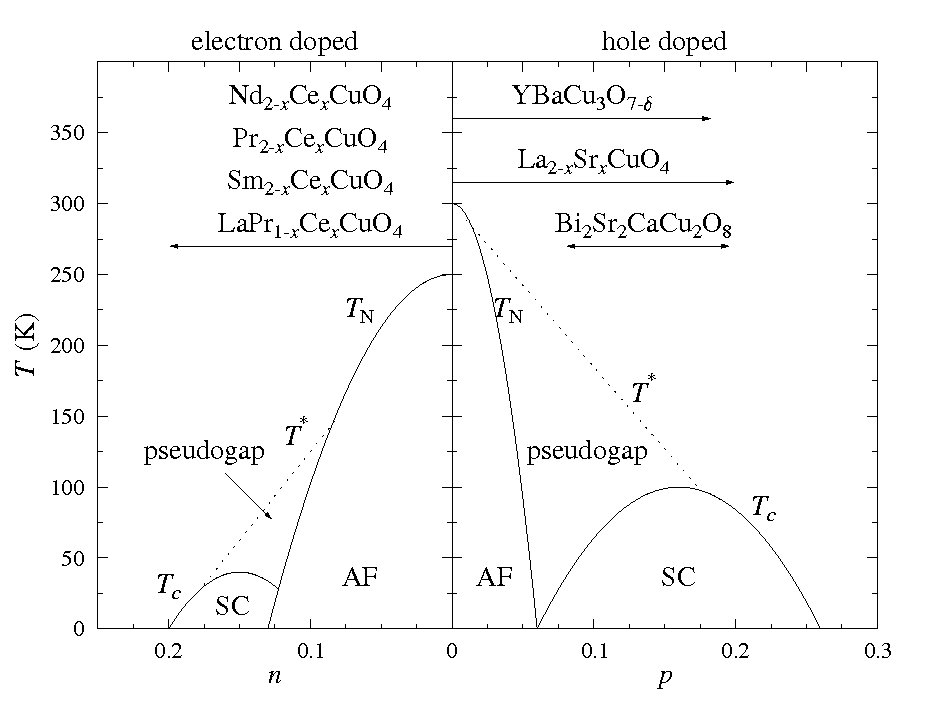
\includegraphics[width=1.0\textwidth]{images/CuPhaseDiag.png}
  \caption{This figure shows a simplified version of the cuprate superconductor phase diagram. \protect\cite{CuPhaseDiag}}
  \label{fig:CuPhaseDiag}
\end{figure}

% Isotopic effects suggested the irrelevance of the lattice, but they are becoming more prominent now.


% First it seemed that in High-Tc the lattice was not that important (isotopic effects at optimal doping).
% Electronic models haven't been completely successful.
In contrast to the BCS theory \cite{Bardeen1957}, the pairing mechanism in the \textit{unconventional superconductors} (cuprates, iron-based and heavy fermion \cite{Pfleiderer2009}) is unknown.
Two leading theories: resonating-valence-bond \cite{?} and spin fluctuation \cite{Scalapino2012} rely heavily on magnetic interactions while mostly ignoring the lattice effects.

% Several experimental observations (lattice and electronic inhomogeneities, phonon spectra and isotopic effects) suggest that lattice plays a fundamental role, altough in a somewhat different fashion than BCS. It seems that below T* there are polaron formation forming the basis state from which superconductivity arises. 

The clues provided by these broken symmetries should yield an understanding of the ground state in this pseudogap phase, its elementary excitations and the appearance of superconductivity at temperatures below the onset of the pseudogap. 

% Electron-lattice correlations could be essential. Maybe in the form of polarons.
% Such correlations can't be adressed with the usual (anti-)adiabatic approximations, so an exact treatment is necessary.
% Exact treatments are computationally expensive so we need to narrow our scope.
% There is evidence of polaronic behaviour in YBCO's O(4)-Cu(1)-O(4).
% A Peierls-Hubbard model has been used there to explain the lattice distortion in terms of bipolarons.
% We explore many other excitations in that model trying to reconcile its predictions with the experimental observations.
% Particular emphasis is given to the isotopic effects because there is controversy around them and they probe the electron-lattice relationship.
% We suggest a possible two-component superconductivity model involving bosonic bi-polaronic objects and free fermions. 
% Chapter outline.


ARPES review: \cite{Damascelli2003}

Pseudogap review: \cite{Timusk1999}

\textit{Inherent inhomogeneity} in HTSC observed by many techniques (see paragraph 2 of \cite{Bussmann-Holder2005}).

The remainder of this introductory chapter is devoted to reviewing some of the experimental results pointing to the importance of considering the lattice and electronic inhomogeneities in the description of superconductivity. 
We start, in section \ref{sec:dynamic_dist} with an overview of the dynamic local lattice distortions in cuprates incluiding the important feature of stripes. 
Afterwards, in section \ref{sec:electronic_inhomogeneity}, we turn our attention to electronic inhomogeneities. 
In sections \ref{sec:phonon_spectra} and \ref{sec:specific_heat} we present some experimental anomalies in the phonon spectra and specific heat respectively and speculate about their possible origin in the mentioned inhomogeneities. 
Next we duscuss some of the controversial experimental results in isotopic effects and ultrafast spectroscopy in sections \ref{sec:isotopic_effects} and \ref{sec:ultrafast_spect} respectively.

In the last part of this introduction we limit the scope of this thesis and present our motivation and approach at describing these dynamic effects (sec. \ref{sec:scope}) and provide an outline of the next chapters (sec. \ref{sec:outline})

\section{Dynamic local lattice distortions}
\label{sec:dynamic_dist}

From https://research-engine.appspot.com/37001/writings/6264610306916352

\begin{quote}
Early determinations of the crystal structure of cuprates by diffraction methods did not show significant distortions associated with either in-plane oxygen atoms or apical oxygen atoms \cite{Capponi1987,Schafer1988}. 
Moreover, the determination of  average bond lengths in diffraction has a precision of $\sim 0.001$\AA \cite{Miceli1988}, significantly higher than the precision in bond length determination that local probes, like extended x-ray absorption fine structure spectroscopy (EXAFS) \cite{Rehr2000}. 
For this reason, early reports of local lattice distortions related to the oxygen atoms  were controversial (see for example \cite{battlog1992lattice,Kwei1990}).

One of the first observations of a local lattice distortion in cuprates was the report of a two-site distribution for the Cu(1)-apical oxygen in YBa$_{2}$Cu$_{3}$O$_{7}$  appearing at temperatures above the superconducting transition temperature, T$_{c}$, using Cu K-edge EXAFS \cite{MustredeLeon1990,Conradson1990}.
This distribution showed two sites separated by $\sim 0.10-0.13$ \AA \cite{Conradson1990,MustredeLeon1992a} that changed into a single site distribution in the vicinity of the superconducting transition temperature. 
These measurements were carried out using polarized x-rays on magnetically oriented powders, an improvement in the technique which allowed to isolate the Cu(1)-axial oxygen [O(4)] (see Fig. 1) signal with an increased sensitivity not achievable for the Cu-O EXAFS signal in other cuprates (see below). 
This result was received with skepticism, based on earlier diffraction results \cite{battlog1992lattice,Kwei1990,Sharma1991} and optical spectroscopy \cite{Thomsen1993}. 
However, it was later confirmed by EXAFS measurements in other oriented samples \cite{Stern1993} and single crystals \cite{Booth1996}, and also found in YBa$_{2}$Cu$_{3}$O$_{6.7}$, YBa$_{2}$Cu$_{3}$O$_{6.5}$ and Co doped YBa$_{2}$Cu$_{3}$O$_{7}$ \cite{MustredeLeon1991}. 
The explanation of the discrepancies between these results with diffraction and optical spectroscopical results lead to the interpretation of  this Cu(1)-O(4) distribution as a dynamical distortion of polaronic origin \cite{MustredeLeon1992}, as discussed in the next section.

Similar two site distributions obtained from EXAFS spectra were found for the Cu(2)-O(4) distribution in Bi$_{2}$Sr$_{2}$CaCu$_{2}$O$_{8}$ \cite{bianconni1992lattice} and in TlBa$_{2}$Ca$_{3}$Cu$_{4}$O$_{11}$ \cite{Allen1991} starting at temperatures above T$_{c}$. 
We note that in these compounds (and other cuprates) the average Cu(2)-O(4) bond length lies between 2.49 and $2.73$ \AA, which is much longer than the Cu(1)-O(4) bond length in YBa$_{2}$Cu$_{3}$O$_{7}$ $(\sim 1.87$ \AA). 
This fact makes more difficult the identification of details of the O(4) distribution due to the stronger mixing of the Cu(2)-O(4) EXAFS signal with those of other atoms and the increased zero point motion of the O(4) atom due to weaker Cu(2)-O(4) bond compared with the Cu(1)-O(4) bond.
For this reason in most EXAFS studies addressing the O(4) motion a gaussian single site broadened distribution has been used, reporting only changes in the width of the distribution as a function of temperature \cite{Booth1995,Oyanagi2007,Zhang2009}.

In plane  Cu(2)-O local lattice distortions were identified in La$_{1.85}$Sr$_{0.15}$CuO$_{4}$ appearing below 100 K \cite{Bianconi1996,Oyanagi2007},  in TIBa$_{2}$CuO$_{6}$ below 120 K \cite{Conradson1997} and in La$_{2}$CuO$_{4.1}$ below 150 K \cite{Lanzara1997,MustredeLeon:xj5003}. 
In this case the observation of such distortions in YBa$_{2}$Cu$_{3}$O$_{7}$ and related compounds becomes more difficult due the similarity  in Cu-O bond lengths in the Cu planes and Cu chains, whose contributions are mixed in the EXAFS signal \cite{Conradson1997,MustredeLeon1992a}.

Until now only in La$_{1.85}$Sr$_{0.15}$CuO$_{4}$ has been possible to identify local lattice distortions involving both in plane oxygen and apical oxygen atoms  \cite{Bianconi1996}. 
We also stress that from all these EXAFS experiments it is only possible to probe with enough detail the nearest neighbor environment around the Cu atoms, thus the spatial extension of the distortions cannot be determined solely from these measurements. 
Additional structural information \cite{Bianconi1996a} is needed to formulate models about the extension of the distortions as discussed in Ref. \cite{Bianconi1996}.

Pair distribution function (PDF) analysis of diffraction, x-ray and neutron inelastic scattering can additionally provide information about the intermediate range (up to $10-15$ \AA)  atomic structure, complementary to the information obtained from EXAFS \cite{Egami2003}. 
PDF results in La$_{1-x}$Sr$_{x}$CuO$_{4}$ \cite{Bozin1999,Bozin2000} indicate that the atomic structure in this material is a combination of nanoscale regions with different local Cu-O environments, in agreement with the model proposed in Ref. \cite{Bianconi1996}. 
A homogeneous structure only appears when dopant concentrations are above $x = 0.25$. 
In this region the electronic behavior can be described in terms of free fermion quasiparticles.

To conclude this survey of local lattice distortion is important to note that the time scale of the EXAFS is such that dynamical distortions can be detected, which depending on the size of the distortion cannot be detected using elastic techniques like neutron diffraction (see section of Results). 
This can explain some of the differences between diffraction and EXAFS results. 
Indeed it has been shown that the two-site O(4) distribution in in Tl$_{2}$Ba$_{2}$CaCu$_{2}$O$_{8}$ could be only detected in a pair distribution function obtained from neutron inelastic scattering but not with that obtained from neutron diffraction \cite{Egami1991}. 
Consequently, it is important to take into account both the spatial resolution and time resolution of the techniques used to study the actual atomic structure of these materials \cite{Mihailovic2005}. 
In the next section we present a microscopic local model that can generate  dynamical local lattice distortions as those observed in these materials, and explain the isotopic effects observed in the pseudogap phase.
\end{quote}

\begin{figure}[ht!]
  \centering
  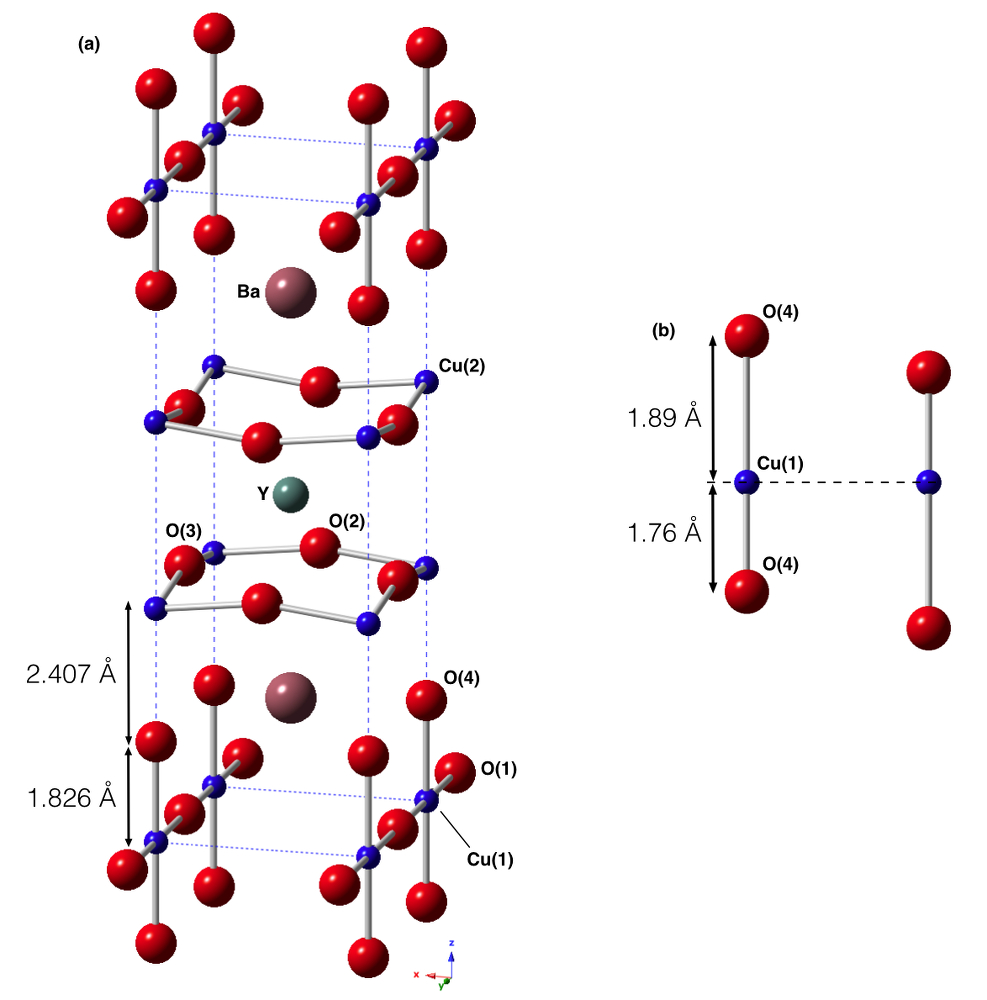
\includegraphics[width=0.8\textwidth]{images/YBCO_O-Cu-O.jpg}
  \caption{\textbf{(a)} Crystal structure of YBa$_{2}$Cu$_{3}$O$_{7}$. The dashed line denotes de unit cell. \textbf{(b)} The two possible configurations in the O(4)-Cu(1)-O(4) cluster due to the split O-Cu bond distances (not to scale).}
\label{fig:YBCO_structure}
\end{figure}

From \cite{Bahrs2004}

\begin{quote}
Samples quenched from high to about room temperature show spontaneous reordering of oxygen atoms in the chain sites on a time scale between hours and days. 
The structural development has been monitored with x-ray and neutron scattering, both verifying a shortening of the crystallographic axes and the formation of superstructure patterns with full and empty chains for values of oxygen deficiency around $\delta \sim  0.5$. 
[...] the critical temperature of the samples was observed to increase, pointing to the close connection between chain length and carrier concentration in the superconducting planes. 
Calculations of the Cu1 valence in different oxygen surroundings explain the charge transfer involved. 
This correlation between structure and electrical properties has also been shown by application of pressure, after which the critical temperature also remains enhanced as long as the sample is kept cool, but relaxes when it is warmed up to room temperature. 
Other metastable effects are induced by illumination, such as persistent photoconductivity, where after exposure to visible light conductivity and, in superconducting samples, critical temperature show a metastable increase.
\end{quote}

\subsection{Stripes}

Review: \cite{Kivelson2003}

\section{Electronic inhomogeneity}
\label{sec:electronic_inhomogeneity}

See introduction of this article: \cite{Ivanov1995}

The parent compounds of cuprate superconductors form ordered crystalline structures and exhibit antiferromagnetic order at low temperatures. 
However,  in compounds like La$_{1.85}$Sr$_{0.15}$CuO$_{4}$ and La$_{2}$CuO$_{4.1}$, the dopant atoms necessary to achieve a superconducting compound are not placed at the crystal symmetry allowed sites yielding to intrinsically structurally inhomogeneous systems\cite{Poccia2011}. 
While in other cases, like YBCO$_{6+\delta}$, extra dopant atoms reside in crystal symmetric positions but the departure from stoichiometry yields compositional disorder\cite{Chen1988} \cite{Andersen1990} with the same consequence. 
In these systems the crystalline translational symmetry is broken. 
Although from the structural inhomogeneity does not necessarily follow an inhomogeneous electronic ground state, for some regions of the phase diagram, depending on the dopant concentration, such state is realized. 
This region of phase space has been identified as the pseudogap phase\cite{Kresin2009} \cite{Muller2007} \cite{Timusk1999}. 
An important consideration is that, although the dopant atoms are at fixed positions, the structural inhomogeneity has a dynamical character\cite{Mihailovic2005} \cite{Bianconi1996} and is present even in compounds with perfect crystallographic symmetry like HoBa$_{2}$Cu$_{4}$O$_{8}$\cite{RubioTemprano2000}. 
In addition to the breaking of the crystalline translational symmetry the pseudogap phase exhibits other broken symmetries. 
Time-reversal symmetry breaking was found using angular resolved photoemission spectroscopy with circularly polarized photons in Bi$_{2}$Sr$_{2}$CaCu$_{2}$O$_{8+\delta}$\cite{Kaminski2002}. 
It was also found, by x-ray absorption spectroscopy, that the crystalline rotational symmetry is broken locally in La$_{1.85}$Sr$_{0.15}$CuO$_{4}$ with alternating regions of tetragonal and orthorhombic symmetry \cite{Bianconi1996}. 
A perspective of the observation of broken symmetries in high-T$_{c}$ superconductors, emphasizing that some of these broken symmetries are hidden from common observational techniques, is discussed in ref.\cite{Chakravarty2011}. The clues provided by these broken symmetries should yield an understanding of the ground state in this pseudogap phase, its elementary excitations and the appearance of superconductivity at temperatures below the onset of the pseudogap. 


\section{Phonon spectra}
\label{sec:phonon_spectra}

Forbidden ir modes only present below T*

\section{Electric resistivity}
\label{sec:resistivity}

T vs T$^2$. See v.g. \cite{Timusk1999}

For a Fermi liquid the dc resistance varies as T$^2$.

\cite{Muller2007}: \textit{At optimum doping, i.e- T$_c$ maximum, and in the normal state, the resistivity increases linearly with temperature}

\section{Specific heat}
\label{sec:specific_heat}

Specific heat: \cite{Loram1993}

For a Fermi liquid the specific heat rises linearly with the temperature.

\section{Isotopic effects}
\label{sec:isotopic_effects}

It is possible to make a site-selective substitution $^{16}$O $\rightarrow$ $^{18}$O in YBCO \cite{Conder1993} allowing a precise study of the isotopic effects. 
This has effects in both the phonon frequencies \cite{Ruani1994} and T$_{c}$ \cite{Zech1994,Cardona1988}. 
The \textit{harmonic} approximation accounts well for the O(2)/O(3) vibrations but it fails for O(4) (see again \cite{Ruani1994})

Noticeable isotopic shifts have been used to identify particular excitations as \textit{phononic} in origin (v.g. \cite{Thomsen1990}) however, we will argue, the converse is not true. 
That is, there can be \textit{phononic} excitations without a measurable isotopic shift.

\section{Ultrafast spectroscopy}
\label{sec:ultrafast_spect}

V.g. \cite{Basov2005} \cite{Smallwood2012} ( http://www.photonics.com/Article.aspx?AID=51474 )

\section{Scope of this thesis}
\label{sec:scope}

% Lattice inhomogeneities limit the applicability of $k$-space formalism.
% Correlated electron-lattice motion prevents the use of Born-Openheimer approximation

Quantum solid-state theory usually assumes a periodic potential however, since these materials are intrinsically inhomogeneous, it is possible that a successful model needs to abandon such assumption. 
This calls into question the applicability of models based on the \textit{reciprocal space} formalism.
Furthermore, some of the experimental results reviewed in the previous secions suggest that the polaronic behaviour must be taken into account.
This correlated electron-lattice movement prevents the use of the Born-Oppenheimer approximation, which splits the system's wavefunction in electronic and lattice factors $\Psi = \psi_{electronic}\psi_{lattice}$.
Some systems with an important electron-lattice interaction can be treated with perturbation theory either assuming a small (adiabatic) or strong (anti-adiabatic) interaction \cite{?}. 
However, it seems that the electron-lattice interaction in the CuO planes for cuprate superconductors falls in the middle of such extremes \cite{MustredeLeon1992} preventing the use of any such approximation.

We are prompted, therefore, to use an exact model free from the approximations described above. 
The computational complexity of exact models forces us to restrict the system under study to a small subset of the whole compound.
In this work we return to a model describing the peculiar polaronic behaviour of the O(4)-Cu(1)-O(4) cluster in YBa$_{2}$Cu$_{3}$O$_{7}$ approximating the cluster as a system with three sites and two holes \cite{MustredeLeon1992}.
Such approximation is justified as the Cu(1)-O(4) bond length (1.83 \AA) is far shorter than the Cu(2)-O(4) bond length ($\sim$ 2.41 \AA) (see Fig. \ref{fig:YBCO_structure}), making charge transfer outside the cluster a much slower process than the charge dynamics inside the cluster. 
This model provides a very simple framework to explore the charge dynamics influenced by the lattice vibrations and has successfully described the split O(4)-Cu(1)-O(4) distance observed by EXAFS experiments (see section \ref{sec:dynamic_dist} above).
Although we cannot directly identify the three site cluster proposed in this model with a particular structure of the CuO plane, the general approach of charge transfer between hole rich regions and hole poor regions in the plane coupled to the lattice degrees of freedom is still valid, hence the general conclusions we draw from this model applicable to describe the structure of the CuO plane.

It has been found that superconductivity occurs in the Cu(2)-O(2,3) planes rather than the Cu(1)-O(1,4) chains partially addressed by the model under study in this work.
This raises a question about the relevance of the polaronic behaviour, es explored with this model, to superconductivity.
It is indeed beyond the capability of such a simple model to address the nature of high-temperature superconductiity.
However, it is possible that the polaronic objects in the Cu(1)-O(1,4) chains are capable of providing a pairing mechanism for the Cooper pairs in the Cu(2)-O(2,3) planes.
This will point to a \textit{two component superconductivity} theory similar to some current proposals \cite{?}

\section{Thesis outline}
\label{sec:outline}

% I need to rewrite this section once I finish everything else...

In chapter \ref{chap:model} we describe in detail the three sites Peierls-Hubbard model used to describe the O-Cu-O cluster in YBCO with some of its generalities. 
The rich phenomenologies of the ground and excited states of this model are explored in the remaining chapters. 
Chapter \ref{chap:ground} is devoted to the ground state (identified also as the \textit{polaron formation energy}). 
Next, in chapter \ref{chap:more_ir}, we describe the next few infrared-allowed excitations. 
Finally, in chapter \ref{chap:electronic}, we turn our attention to the first \textit{electronic} excitation of this model. 
We conclude this work, in chapter \ref{chap:conclusions}, with some conclusions and perspectives.
